\section{The product and quotient rules} \label{S:2.5.ProdQuot}

\begin{goals}
\item How does the algebraic structure of a function direct us in computing its derivative using shortcut rules?
\item How do we compute the derivative of a product of two basic functions in terms of the derivatives of the basic functions?
\item How do we compute the derivative of a quotient of two basic functions in terms of the derivatives of the basic functions?
\item How do the product and quotient rules combine with the sum and constant multiple rules to expand the library of functions we can quickly differentiate?
\item What are the derivatives of the tangent, cotangent, secant, and cosecant functions?
\item How do the derivatives of $\tan(x)$, $\cot(x)$, $\sec(x)$, and $\csc(x)$ combine with other derivative rules we have developed to expand the library of functions we can quickly differentiate?
\end{goals}

%--------------------------------------
% SUBSECTION INTRODUCTION
%--------------------------------------
\subsection*{Introduction}

So far, the basic functions we know how to differentiate include power functions ($x^n$), exponential functions ($a^x$), and the two fundamental trigonometric functions ($\sin(x)$ and $\cos(x)$).  With the sum rule and constant multiple rules, we can also compute the derivative of combined functions such as
$$f(x) = 7x^{11} - 4 \cdot 9^x + \pi \sin(x) - \sqrt{3}\cos(x),$$
because the function $f$ is fundamentally a sum of basic functions.  Indeed, we can now quickly say that $f'(x) = 77x^{10} - 4 \cdot 9^x \ln(9) + \pi \cos(x) + \sqrt{3} \sin(x)$.  

But we can of course combine basic functions in ways other than multiplying them by constants and taking sums and differences.  For example, we could consider the function that results from a product of two basic functions, such as $$p(z) = z^3 \cos(z),$$
or another that is generated by the quotient of two basic functions, one like
$$q(t) = \frac{\sin(t)}{2^t}.$$
While the derivative of a sum is the sum of the derivatives, it turns out that the rules for computing derivatives of products and quotients are more complicated.  In what follows we explore why this is the case, what the product and quotient rules actually say, and work to expand our repertoire of functions we can easily differentiate.  To start, Preview Activity~\ref{PA:2.5} asks you to investigate the derivative of a product and quotient of two polynomials.

\begin{pa} \label{PA:2.5}
Let $f$ and $g$ be the functions defined by $f(t) = 2t^2$ and $g(t) = t^3 + 4t$.
\ba
	\item Determine $f'(t)$ and $g'(t)$.
	\item Let $p(t) = 2t^2 (t^3 + 4t)$ and observe that $p(t) = f(t) \cdot g(t)$.  Rewrite the formula for $p$ by distributing the $2t^2$ term.  Then, compute $p'(t)$ using the sum and constant multiple rules.
	\item True or false: $p'(t) = f'(t) \cdot g'(t)$.  
	\item Let $\ds q(t) = \frac{t^3 + 4t}{2t^2}$ and observe that $\ds q(t) = \frac{g(t)}{f(t)}$.  Rewrite the formula for $q$ by dividing each term in the numerator by the denominator and simplify to write $q$ as a sum of constant multiples of powers of $t$.  Then, compute $q'(t)$ using the sum and constant multiple rules.
	\item True or false: $\ds q'(t) = \frac{g'(t)}{f'(t)}$.  
\ea

\end{pa} \afterpa % PREVIEW ACTIVITY

%-----------------------------------
% SUBSECTION PRODUCT RULE
%-----------------------------------
\subsection*{The product rule}

As parts (b) and (d) of Preview Activity~\ref{PA:2.5} show, it is not true in general that the derivative of a product of two functions is the product of the derivatives of those functions.  Indeed, the rule for differentiating a function of the form $p(x) = f(x) \cdot g(x)$ in terms of the derivatives of $f$ and $g$ is more complicated than simply taking the product of the derivatives of $f$ and $g$.  To see further why this is the case, as well as to begin to understand how the product rule actually works, we consider an example involving meaningful functions.

Say that an investor is regularly purchasing stock in a particular company.  Let $N(t)$ be a function that represents the number of shares owned on day $t$, where $t = 0$ represents the first day on which shares were purchased.  Further, let $S(t)$ be a function that gives the value of one share of the stock on day $t$; note that the units on $S(t)$ are dollars per share.  Moreover, to compute the total value on day $t$ of the stock held by the investor, we use the function $V(t) = N(t) \cdot S(t)$.  By taking the product 
$$V(t) = N(t) \, \mbox{shares} \cdot S(t) \, \mbox{dollars per share},$$ 
we have the total value in dollars of the shares held.  Observe that over time, both the number of shares and the value of a given share will vary.  The derivative $N'(t)$ measures the rate at which the number of shares held is changing, while $S'(t)$ measures the rate at which the value per share is changing.  The big question we'd like to answer is: how do these respective rates of change affect the rate of change of the total value function?

To help better understand the relationship among changes in $N$, $S$, and $V$, let's consider some specific data.  Suppose that on day $100$, the investor owns $520$ shares of stock and the stock's current value is $\$27.50$ per share.  This tells us that $N(100) = 520$ and $S(100) = 27.50$.  In addition, say that on day $100$, the investor purchases an additional $12$ shares (so the number of shares held is rising at a rate of $12$ shares per day), and that on that same day the price of the stock is rising at a rate of $0.75$ dollars per share per day.  Viewed in calculus notation, this tells us that $N'(100) = 12$ (shares per day) and $S'(100) = 0.75$ (dollars per share per day).  At what rate is the value of the investor's total holdings changing on day $100$?

Observe that the increase in total value comes from two sources: the growing number of shares, and the rising value of each share.  If only the number of shares is rising (and the value of each share is constant), the rate at which which total value would rise is found by computing the product of the current value of the shares with the rate at which the number of shares is changing.  That is, the rate at which total value would change is given by \small
\[ S(100) \cdot N'(100) = 27.50 \, \frac{\mbox{dollars}}{\mbox{share}} \cdot 12 \, \frac{\mbox{shares}}{\mbox{day}} = 330 \, \frac{\mbox{dollars}}{\mbox{day}}.\] \normalsize
Note particularly how the units make sense and explain that we are finding the rate at which the total value $V$ is changing, measured in dollars per day.  If instead the number of shares is constant, but the value of each share is rising, then the rate at which the total value would rise is found similarly by taking the product of the number of shares with the rate of change of share value.  In particular, the rate total value is rising is \small
\[ N(100) \cdot S'(100) = 520 \, \mbox{shares} \cdot 0.75 \, \frac{\mbox{dollars per share}}{\mbox{day}} = 390 \, \frac{\mbox{dollars}}{\mbox{day}}. \] \normalsize
Of course, when both the number of shares is changing and the value of each share is changing, we have to include both of these sources, and hence the rate at which the total value is rising is \small
\begin{align*}
V'(100) & = S(100) \cdot N'(100) + N(100) \cdot S'(100) \\
& = 330 + 390 = 720 \, \frac{\mbox{dollars}}{\mbox{day}}.
\end{align*}\normalsize

This tells us that we expect the total value of the investor's holdings to rise by about $\$720$ on the 100th day.\sidenote[][-4cm]{While this example highlights why the product rule is true, there are some subtle issues to recognize.  For one, if the stock's value really does rise exactly $\$0.75$ on day $100$, and the number of shares really rises by $12$ on day $100$, then we'd expect that $V(101) = N(101) \cdot S(101) = 532 \cdot 28.25 = 15029$.  If, as noted above, we expect the total value to rise by $\$720$, then with $V(100) = N(100) \cdot S(100) = 520 \cdot 27.50 = 14300$, then it seems like we should find that $V(101) = V(100) + 720 = 15020.$  Why do the two results differ by $9$?  One way to understand why this difference occurs is to recognize that $N'(100) = 12$ represents an \emph{instantaneous} rate of change, while our (informal) discussion has also thought of this number as the total change in the number of shares over the course of a single day.  The formal proof of the product rule reconciles this issue by taking the limit as the change in the input tends to zero.}

Next, we expand our perspective from the specific example above to the more general and abstract setting of a product $p$ of two differentiable functions, $f$ and $g$.  If we have $P(x) = f(x) \cdot g(x)$, our work above suggests that $P'(x) = f(x) g'(x) + g(x) f'(x).$ Indeed, a formal proof using the limit definition of the derivative can be given to show that the following rule, called the \emph{product rule}\index{product rule}, holds in general.

\concept{ Product Rule \index{product rule}}{ % CONCEPT
If $f$ and $g$ are differentiable functions, then their product $P(x) = f(x) \cdot g(x)$ is also a differentiable function, and
\[ P'(x) = f(x) g'(x) + g(x) f'(x). \]
} %end concept

\begin{example} \label{Ex:2.5.Eg1}
Use the definition of the derivative to prove the Product Rule for differentiation.

\solution By the limit definition, we have 
\[ \frac{d}{dx}\Big(f(x)g(x)\Big) =\lim_{h \to 0} \frac{f(x+h)g(x+h)-f(x)g(x)}{h}.\] 
We now do something a bit unexpected; add $0$ to the numerator (so that nothing is changed) in the form of $-f(x+h)g(x)+f(x+h)g(x)$, then do some regrouping as shown.
\begin{align*}
\left.\right.& \frac{d}{dx}\Big(f(x)g(x)\Big) \\
&=\lim_{h\to0} \frac{f(x+h)g(x+h)-f(x)g(x)}{h} \quad \parbox{120pt}{ (now add $0$ to the numerator) } \\
&=	\lim_{h\to0} \frac{f(x+h)g(x+h)-f(x+h)g(x)+f(x+h)g(x)-f(x)g(x)}{h} \\ % \quad \parbox{100pt}{\small (regroup)} \\
&=	\lim_{h\to0} \frac{\Big(f(x+h)g(x+h)-f(x+h)g(x)\Big)+\Big(f(x+h)g(x)-f(x)g(x)\Big)}{h}\\
&=	\lim_{h\to0} \frac{f(x+h)g(x+h)-f(x+h)g(x)}{h}+\lim_{h\to0}\frac{f(x+h)g(x)-f(x)g(x)}{h} \\ %\quad\parbox{100pt}{\small (factor)}\\
&=\lim_{h\to0} f(x+h)\frac{g(x+h)-g(x)}{h}+\lim_{h\to0}\frac{f(x+h)-f(x)}{h}g(x) \\ %\quad\parbox{100pt}{\small (apply limits)}\\
&=f(x)g'(x) + \fp(x)g(x)
\end{align*}
\end{example} %EXAMPLE (PRODUCT RULE PROOF)

In light of the earlier example involving shares of stock, the product rule also makes sense intuitively:  the rate of change of $P$ should take into account both how fast $f$ and $g$ are changing, as well as how large $f$ and $g$ are at the point of interest.  Furthermore, we note in words what the product rule says:  if $P$ is the product of two functions $f$ (the first function) and $g$ (the second), then "the derivative of $P$ is the first times the derivative of the second, plus the second times the derivative of the first."  It is often a helpful mental exercise to say this phrasing aloud when executing the product rule.

\begin{example} \label{Ex:2.5.Eg3}
Use the Product Rule to compute the derivative of $P(z) = z^3 \cdot \cos(z)$. 

\solution The first function is $z^3$ and the second function is $\cos(z)$.  By the product rule, $P'$ will be given by the first, $z^3$, times the derivative of the second, $-\sin(z)$, plus the second, $\cos(z)$, times the derivative of the first,  $3z^2$.  That is,
\[ P'(z) = z^3(-\sin(z)) + \cos(z) 3z^2 = -z^3 \sin(z) + 3z^2 \cos(z).\]
\end{example} % EXAMPLE

The following activity further explores the use of the product rule.

\begin{activity} \label{A:2.5.1}  Use the product rule to answer each of the questions below.  Throughout, be sure to carefully label any derivative you find by name.  That is, if you're given a formula for $f(x)$, clearly label the formula you find for $f'(x)$.  It is not necessary to algebraically simplify any of the derivatives you compute.
\ba
	\item Let $m(w)=3w^{17} 4^w$.  Find $m'(w)$.
	\item Let $h(t) = (\sin(t) + \cos(t))t^4$.  Find $h'(t)$.
	\item Determine the slope of the tangent line to the curve $y = f(x)$ at the point where $a = 1$ if $f$ is given by the rule $f(x) = e^x \sin(x)$.
	\item Find the tangent line approximation $L(x)$ to the function $y = g(x)$ at the point where $a = -1$ if $g$ is given by the rule $g(x) = (x^2 + x) 2^x$.
\ea

\end{activity}
\begin{smallhint}
\ba
	\item Let the first function be $3w^{17}$.
	\item Let the first function be $(\sin(t) + \cos(t))$.
	\item Remember that the slope of the tangent line to $y = f(x)$ at $(a,f(a))$ is given by $f'(a)$.
	\item Remember that $L(x) = g(a) + g'(a)(x-a).$
\ea
\end{smallhint}
\begin{bighint}
\ba
	\item Let the first function be $3w^{17}$ and the second function be $4^w$.
	\item Let the first function be $(\sin(t) + \cos(t))$ and the second function be $t^4$.
	\item Remember that the slope of the tangent line to $y = f(x)$ at $(a,f(a))$ is given by $f'(a)$.
	\item Remember that $L(x) = g(a) + g'(a)(x-a).$  In differentiating $g$, let the first function be $(x^2 + x)$.
\ea
\end{bighint}
\begin{activitySolution}
\ba
	\item By the product rule, 
	$$m'(w) = 3w^{17} \cdot 4^w \ln(4) + 4^w \cdot 3w^17.$$ 
	\item By the product rule, 
	$$h'(t) = (\sin(t) + \cos(t)) \cdot 4t^3 + t^4 \cdot (\cos(t) - \sin(t)).$$ 
	\item To determine the slope of the tangent line at $a = 1$, we want to find $f'(1)$.  Since $f(x) = e^x \sin(x)$, the product rule tells us that $f'(x) = e^x \cdot \cos(x) + \sin(x) \cdot e^x$.  Thus, $f'(1) = e^1 \cdot \cos(1) + \sin(1) \cdot e^1 = e(\cos(1) + \sin(1)) \approx 3.756$.
	\item First, observe that $g(-1) = ((-1)^2 - 1) \cdot 2^{-1} = 0$.  Further, by the product rule, $g'(x) = (x^2 + x) \cdot 2^x \ln(2) + 2^x \cdot (2x + 1)$, and therefore $g'(-1) = ((-1)^2 - 1) \cdot 2^{-1} \ln(2) + 2^{-1} \cdot (2(-1) + 1) = 0 + \frac{1}{2}(-1) = -\frac{1}{2}.$  Therefore,
	$$L(x) = g(-1) + g'(-1)(x+1) = 0 - \frac{1}{2}(x+1) = -\frac{1}{2}(x+1).$$
\ea
\end{activitySolution}
\aftera %ACTIVITY

%---------------------------------------
% SUBSECTION QUOTIENT RULE
%---------------------------------------
\subsection*{The quotient rule}

Because quotients and products are closely linked, we can use the product rule to understand how to take the derivative of a quotient.  In particular, let $Q(x)$ be defined by $Q(x) = f(x)/g(x)$, where $f$ and $g$ are both differentiable functions.  We desire a formula for $Q'$ in terms of $f$, $g$, $f'$, and $g'$.  It turns out that $Q$ is differentiable everywhere that $g(x) \ne 0$.  Moreover, taking the formula $Q = f/g$ and multiplying both sides by $g$, we can observe that 
\[ f(x) = Q(x) \cdot g(x). \]
Thus, we can use the product rule to differentiate $f$.  Doing so,
\[ f'(x) = Q(x) g'(x) + g(x) Q'(x).\]
Since we want to know a formula for $Q'$, we work to solve this most recent equation for $Q'(x)$, finding first that
\[ Q'(x) g(x) = f'(x) - Q(x) g'(x).\]
Dividing both sides by $g(x)$, we have
\[ Q'(x) = \frac{f'(x) - Q(x) g'(x)}{g(x)}.\]
Finally, we also recall that $Q(x) = \frac{f(x)}{g(x)}.$  Using this expression in the preceding equation and simplifying, we have
\begin{eqnarray*}
Q'(x) & = & \frac{f'(x) - \frac{f(x)}{g(x)} g'(x)}{g(x)} \\
	& = & \frac{f'(x) - \frac{f(x)}{g(x)} g'(x)}{g(x)} \cdot \frac{g(x)}{g(x)} \\
	& = & \frac{g(x) f'(x) -  f(x) g'(x)}{g(x)^2}. 
\end{eqnarray*}
This shows the fundamental argument for why the \emph{quotient rule} holds.

\concept{ Quotient Rule \index{quotient rule}}{ % CONCEPT
If $f$ and $g$ are differentiable functions, then their quotient $Q(x) = \frac{f(x)}{g(x)}$ is also a differentiable function for all $x$ where $g(x) \ne 0$, and
\[ Q'(x) = \frac{g(x)f'(x) - f(x) g'(x)}{g(x)^2}.\]
} %end concept

Like the product rule, it can be helpful to think of the quotient rule verbally.  If a function $Q$ is the quotient of a top function $f$ and a bottom function $g$, then $Q'$ is given by ``the bottom times the derivative of the top, minus the top times the derivative of the bottom, all over the bottom squared.''  

\begin{example} \label{Ex:2.5.Eg4}
Use the Quotient Rule to compute the derivative of $Q(t) = \sin(t)/2^t$. 

\solution We can identify the top function as $\sin(t)$ and the bottom function as $2^t$.  By the quotient rule, we then have that $Q'$ will be given by the bottom, $2^t$, times the derivative of the top, $\cos(t)$, minus the top, $\sin(t)$, times the derivative of the bottom, $2^t \ln(2)$, all over the bottom squared, $(2^t)^2$.  That is,
\[ Q'(t) = \frac{2^t \cos(t) - \sin(t) 2^t \ln(2)}{(2^t)^2}.\]

In this particular example, it is possible to simplify $Q'(t)$ by removing a factor of $2^t$ from both the numerator and denominator, hence finding that
\[ Q'(t) = \frac{\cos(t) - \sin(t) \ln(2)}{2^t}. \]
In general, we must be careful in doing any such simplification, as we don't want to correctly execute the quotient rule but then find an incorrect overall derivative due to an algebra error.  As such, we will often place more emphasis on correctly using derivative rules than we will on simplifying the result that follows.
\end{example} %EXAMPLE

The following activity further explores the use of the quotient rule.

\begin{activity} \label{A:2.5.2} Use the quotient rule to answer each of the questions below.  Throughout, be sure to carefully label any derivative you find by name.  
That is, if you're given a formula for $f(x)$, clearly label the formula you find for $f'(x)$.  It is not necessary to algebraically simplify any of the derivatives you compute.
\ba
	\item Let $\ds r(z)=\frac{3^z}{z^4 + 1}$.  Find $r'(z)$.
	\item Let $\ds v(t) = \frac{\sin(t)}{\cos(t) + t^2}$.  Find $v'(t)$.
	\item Determine the slope of the tangent line to the curve $\displaystyle R(x) = \frac{x^2 - 2x - 8}{x^2 - 9}$ at the point where $x = 0$.
	\item When a camera flashes, the intensity $I$ of light seen by the eye is given by the function
$$I(t) = \frac{100t}{e^t},$$
where $I$ is measured in candles and $t$ is measured in milliseconds.  Compute $I'(0.5)$, $I'(2)$, and $I'(5)$; include appropriate units on each value; and discuss the meaning of each.
\ea
\end{activity}
\begin{smallhint}
\ba
	\item When applying the quotient rule, use parentheses around the bottom function, $z^4 + 1$, to ensure that when you compute ``the bottom times the derivative of the top'' that the rule is applied correctly.
	\item When applying the quotient rule, use parentheses around the bottom function, $\cos(t) + t^2$, and its derivative to ensure that the rule is applied correctly.
	\item Remember one of the key interpretations of the derivative.
	\item Let the top function be $100t$ and simply use the constant multiple rule to find its derivative.
\ea
\end{smallhint}
\begin{bighint}
\ba
	\item When applying the quotient rule, use parentheses around the bottom function, $z^4 + 1$, to ensure that when you compute ``the bottom times the derivative of the top'' that the rule is applied correctly.
	\item When applying the quotient rule, use parentheses around the bottom function, $\cos(t) + t^2$, and its derivative to ensure that the rule is applied correctly.
	\item Remember that the derivative evaluated at a particular value gives the slope of the tangent line there.
	\item Let the top function be $100t$ and simply use the constant multiple rule to find its derivative.  Further, note that since the units on $I$ are candles and those on $t$ are milliseconds, the units on $I'(t)$ will be candles per millisecond.
\ea
\end{bighint}
\begin{activitySolution}
\ba
	\item By the quotient rule,
	$$r'(z)=\frac{(z^4+1) 3^z \ln(3) - 3^z(4z^3)}{(z^4 + 1)^2}.$$
	\item By the quotient rule, 
	$$v'(t) = \frac{(\cos(t) + t^2)\cos(t) - \sin(t)(\sin(t) + 2t)}{(\cos(t) + t^2)^2}.$$
	\item We first compute $R'(x)$.  By the quotient rule,
	$$R'(x) = \frac{(x^2 - 9)(2x - 2) - (x^2 - 2x - 8)(2x)}{(x^2 - 9)^2}.$$
	From this, it follows that $R'(0) = \frac{(-9)(-2)-(-8)(0)}{(-9)^2} = -\frac{2}{9}$, which is the slope of the tangent line to the curve at the point where $x = 0$.
	\item By the quotient rule and algebraic simplification,
$$I'(t) = \frac{e^t 100 - 100te^t}{(e^t)^2} = \frac{100-100t}{e^t}.$$
Thus, $I'(0.5) = \frac{50}{e^{0.5}} \approx 30.327$, $I'(2) = \frac{-100}{e^{2}} \approx -13.534$, and $I'(5) = \frac{-400}{e^4} \approx -2.695$, each measured in candles per millisecond.  These results show that at $t = 0.5$, the intensity of the flash is increasing rapidly, while at $t = 2$ and $t = 5$, the intensity is decreasing, with the intensity decreasing more rapidly when $t = 2$.
\ea
\end{activitySolution}
\aftera %ACTIVITY

%------------------------------------------
% SUBSECTION COMBINING RULES
%------------------------------------------
\subsection*{Combining rules}

One of the challenges to learning to apply various derivative shortcut rules correctly and effectively is recognizing the fundamental structure of a function.  For instance, consider the function given by
$$f(x) = x\sin(x) + \frac{x^2}{\cos(x) + 2}.$$
How do we decide which rules to apply?  Our first task is to recognize the overall structure of the given function.  Observe that the function $f$ is fundamentally a sum of two slightly less complicated functions, so we can apply the sum rule\sidenote[][-2cm]{When taking a derivative that involves the use of multiple derivative rules, it is often helpful to use the notation $\frac{d}{dx} \left[ ~~\right]$ to wait to apply subsequent rules.  This is demonstrated in each of the two examples presented here.} and get
\begin{eqnarray*}
f'(x) & = & \frac{d}{dx} \left[ x\sin(x) + \frac{x^2}{\cos(x) + 2} \right] \\
	& = & \frac{d}{dx} \left[ x\sin(x) \right] + \frac{d}{dx}\left[ \frac{x^2}{\cos(x) + 2} \right]  
\end{eqnarray*}
Now, the left-hand term above is a product, so the product rule is needed there, while the right-hand term is a quotient, so the quotient rule is required.  Applying these rules respectively, we find that
\begin{eqnarray*}
 f'(x) & = & \left( x \cos(x) + \sin(x) \right) + \frac{(\cos(x) + 2) 2x - x^2(-\sin(x))}{(\cos(x) + 2)^2} \\
        & = & x \cos(x) + \sin(x) + \frac{2x\cos(x) + 4x^2 + x^2\sin(x)}{(\cos(x) + 2)^2}.
\end{eqnarray*}

We next consider how the situation changes with the function defined by
$$s(y) = \frac{y \cdot 7^y}{y^2 + 1}.$$ 
Overall, $s$ is a quotient of two simpler function, so the quotient rule will be needed.  Here, we execute the quotient rule and use the notation $\frac{d}{dy}$ to defer the computation of the derivative of the numerator and derivative of the denominator.  Thus,
$$s'(y) = \frac{(y^2 + 1) \cdot \frac{d}{dy}\left[ y \cdot 7^y \right] - y \cdot 7^y \cdot \frac{d}{dy}\left[y^2 + 1 \right]}{(y^2 + 1)^2}.$$
Now, there remain two derivatives to calculate.  The first one, $\frac{d}{dy}\left[ y \cdot 7^y \right]$ calls for use of the product rule, while the second, $\frac{d}{dy}\left[y^2 + 1 \right]$ takes only an elementary application of the sum rule.  Applying these rules, we now have
$$s'(y) = \frac{(y^2 + 1) [y \cdot 7^y \ln(7) + 7^y \cdot 1] - y \cdot 7^y [2y]}{(y^2 + 1)^2}.$$
While some minor simplification is possible, we are content to leave $s'(y)$ in its current form, having found the desired derivative of $s$.  In summary, to compute the derivative of $s$, we applied the quotient rule.  In so doing, when it was time to compute the derivative of the top function, we used the product rule; at the point where we found the derivative of the bottom function, we used the sum rule.

In general, one of the main keys to success in applying derivative rules is to recognize the structure of the function, followed by the careful and diligent application of relevant derivative rules.  The best way to get good at this process is by doing a large number of exercises, and the next activity provides some practice and exploration to that end.

\begin{activity} \label{A:2.5.3} Use relevant derivative rules to answer each of the questions below.  Throughout, be sure to use proper notation and carefully label any derivative you find by name.  
\ba
	\item Let $\ds f(r) = (5r^3 + \sin(r))(4^r - 2\cos(r))$.  Find $f'(r)$.  
	\item Let $\displaystyle p(t) = \frac{\cos(t)}{t^6 \cdot 6^t}$.  Find $p'(t)$.
	\item Let $\ds g(z) = 3z^7 e^z - 2z^2 \sin(z) + \frac{z}{z^2 + 1}.$  Find $g'(z)$.
	\item A moving particle has its position in feet at time $t$ in seconds given by the function $\ds s(t) = \frac{3\cos(t) - \sin(t)}{e^t}$.  Find the particle's instantaneous velocity at the moment $t = 1$.
	\item Suppose that $f(x)$ and $g(x)$ are differentiable functions and it is known that $f(3) = -2$, $f'(3) = 7$, $g(3) = 4$, and  $g'(3) = -1$.  If $p(x) = f(x) \cdot g(x)$ and $\displaystyle q(x) = \frac{f(x)}{g(x)}$, calculate $p'(3)$ and $q'(3)$.
\ea
\end{activity}
\begin{smallhint}
\ba
	\item Observe that $f$ is fundamentally a product.  Which is the first function?  The second?  
	\item Note that $p$ has the overall structure of a quotient.
	\item Think about how $g$ is a sum of three functions.  What is the structure of each of the three functions in the sum?
	\item How is the velocity of a moving object related to its position?
	\item Since we know $p(x) = f(x) \cdot g(x)$, it follows $p'(x) = f(x) g'(x) + g(x) f'(x).$
\ea
\end{smallhint}
\begin{bighint}
\ba
	\item Observe that $f$ is fundamentally a product.  Which is the first function?  The second?  What rule(s) are needed to differentiate the first function?  The second? 
	\item Note that $p$ has the overall structure of a quotient.  What is the structure of the bottom function?
	\item Think about how $g$ is a sum of three functions.  What is the structure of each of the three functions in the sum?
	\item How is the velocity of a moving object related to its position?  What is the structure of $s(t)$?
	\item Since we know $p(x) = f(x) \cdot g(x)$, it follows $p'(x) = f(x) g'(x) + g(x) f'(x)$ for any value of $x$.  How can you use the given information?
\ea
\end{bighint}
\begin{activitySolution}
\ba
	\item Using the product rule, followed by the sum and constant multiple rule, observe that
	\begin{eqnarray*}
	f'(r) & = & (5r^3 + \sin(r))\frac{d}{dr}[4^r - 2\cos(r)] +  (4^r - 2\cos(r))\frac{d}{dr}[5r^3 + \sin(r)] \\
	      & = &  (5r^3 + \sin(r))[4^r \ln(4) + 2\sin(r)] +  (4^r - 2\cos(r))[15r^2 + \cos(r)]
	\end{eqnarray*}
	\item We use the quotient rule on $p$, followed by the product rule to differentiate the denominator, finding that
	\begin{eqnarray*}
	  p'(t) & = & \frac{t^6 \cdot 6^t \frac{d}{dt}[\cos(t)] - \cos(t) \frac{d}{dt}[t^6 \cdot 6^t]}{(t^6 \cdot 6^t)^2} \\
	         & = & \frac{t^6 \cdot 6^t [-\sin(t)] - \cos(t) [t^6 \cdot 6^t \ln(6) + 6^t \cdot 6t^5]}{(t^6 \cdot 6^t)^2}
	\end{eqnarray*}
		
	\item Using the sum and constant multiple rules, it follows first that
	$$g'(z) = 3 \frac{d}{dz}[z^7 e^z] - 2\frac{d}{dz}[z^2 \sin(z)] + \frac{d}{dz}\left[ \frac{z}{z^2 + 1} \right].$$  
	Applying the product rule in the first two terms and the quotient rule in the third, we find that
	$$g'(z) = 3 [z^7 e^z +  7z^6e^z] - 2[z^2 \cos(z) + 2z\sin(z)] + \frac{(z^2+1) 1 - z(2z)}{(z^2 + 1)^2}.$$  

	\item The particle's instantaneous velocity at the moment $t = 1$ is given by $s'(1)$.  We use the quotient rule to find $s'(t)$, and simplify by removing a common factor of $e^t$ to get
	$$s'(t) = \frac{e^t(-3\sin(t) - \cos(t))-(3\cos(t) - \sin(t))e^t}{(e^t)^2} = \frac{-2\sin(t)-4\cos(t)}{e^t}.$$
	Thus, $s'(1) = \frac{-2\sin(1)-4\cos(1)}{e^1} \approx -1.414$, which is the particle's instantaneous velocity in feet per second at the moment $t = 1$.
	\item Since $p(x) = f(x) \cdot g(x)$, the product rule tells us
	$$p'(x) = f(x)g'(x) + g(x)f'(x),$$
	and since $\displaystyle q(x) = \frac{f(x)}{g(x)}$, by the quotient rule we know
	$$q'(x) = \frac{g(x)f'(x)-f(x)g'(x)}{g(x)^2}.$$
	Using the given information ($f(3) = -2$, $f'(3) = 7$, $g(3) = 4$, and  $g'(3) = -1$) we now see that
	$$p'(3) = f(3)g'(3) + g(3)f'(3) = (-2)(-1) + (4)(7) = 30$$
	and
	$$q'(x) = \frac{g(3)f'(3)-f(3)g'(3)}{g(3)^2} = \frac{(4)(7) - (-2)(-1)}{4^2} = \frac{13}{8}.$$
\ea
\end{activitySolution}
\aftera %ACTIVITY

As the algebraic complexity of the functions we are able to differentiate continues to increase, it is important to remember that all of the derivative's meaning continues to hold.  Regardless of the structure of the function $f$, the value of $f'(a)$ tells us the instantaneous rate of change of $f$ with respect to $x$ at the moment $x = a$, as well as the slope of the tangent line to $y = f(x)$ at the point $(a,f(a))$.

%--------------------------------------------------
% SUBSECTION OTHER TRIG FUNCTIONS
%--------------------------------------------------
\subsection*{Derivatives of the tangent, cotangent, secant, and cosecant functions} \index{cotangent} \index{secant} \index{cosecant}

\begin{activity} \label{A:2.5.Act4}
Consider the function $\ds f(x) = \tan(x)$, and remember that $\ds \tan(x) = \frac{\sin(x)}{\cos(x)}$.
\ba
	\item What is the domain of $f$?
	\item Use the quotient rule to show that one expression for $f'(x)$ is
	$$f'(x) = \frac{\cos(x)\cos(x) + \sin(x)\sin(x)}{\cos^2(x)}.$$
	\item What is the Fundamental Trigonometric Identity?  How can this identity be used to find a simpler form for $f'(x)$?
	\item Recall that $\ds \sec(x) = \frac{1}{\cos(x)}$.  How can we express $f'(x)$ in terms of the secant function?
	\item For what values of $x$ is $f'(x)$ defined?  How does this set compare to the domain of $f$?
\ea
\end{activity} 
%\afterpa %ACTIVITY

In Activity~\ref{A:2.5.Act4}, we found that the derivative of the tangent function can be expressed in several ways, but most simply in terms of the secant function.  Next, we develop the derivative of the cotangent function.

Let $g(x) = \cot(x)$.  To find $g'(x)$, we observe that $g(x) = \frac{\cos(x)}{\sin(x)}$ and apply the quotient rule.  Hence
\begin{eqnarray*}
	g'(x) & = & \frac{\sin(x)(-\sin(x)) - \cos(x) \cos(x)}{\sin^2(x)} \\
	        & = & -\frac{\sin^2(x) + \cos^2(x)}{\sin^2(x)}
\end{eqnarray*}
By the Fundamental Trigonometric Identity, we see that $g'(x) = -\frac{1}{\sin^2(x)}$; recalling that $\csc(x) = \frac{1}{\sin(x)}$, it follows that we can most simply express $g'$ by the rule
$$g'(x) = -\csc^2(x).$$
Note that neither $g$ nor $g'$ is defined when $\sin(x) = 0$, which occurs at every integer multiple of $\pi$.  Hence we have the following rule.

\concept{ Cotangent Function \index{derivative!cotangent}}{ % CONCEPT
For all real numbers $x$ such that $x \ne k\pi$, where $k = 0,$ $\pm 1,$ $\pm 2, \ldots$,  
\[ \frac{d}{dx} [\cot(x)] = -\csc^2(x). \]
} %end concept

Observe that the shortcut rule for the cotangent function is very similar to the rule we discovered in Activity~\ref{A:2.5.Act4} for the tangent function.

\concept{ Tangent Function \index{derivative!tangent}}{  % CONCEPT
For all real numbers $x$ such that $x \ne \frac{k\pi}{2}$, where $k = \pm 1,$ $\pm 2, \ldots$,  
\[ \frac{d}{dx} [\tan(x)] = \sec^2(x). \]
} %end concept

In the next two activities, we develop the rules for differentiating the secant and cosecant functions.

\begin{activity} \label{A:2.5.5}  
Let $h(x) = \sec(x)$ and recall that $\ds \sec(x) = \frac{1}{\cos(x)}$.
\ba
	\item What is the domain of $h$?
	\item Use the quotient rule to develop a formula for $h'(x)$ that is expressed completely in terms of $\sin(x)$ and $\cos(x)$.
	\item How can you use other relationships among trigonometric functions to write $h'(x)$ only in terms of $\tan(x)$ and $\sec(x)$?
	\item What is the domain of $h'$?  How does this compare to the domain of $h$? 
\ea
\end{activity}
\begin{smallhint}
\ba
	\item For what values of $x$ is $\cos(x) = 0$?
	\item Don't forget that $\frac{d}{dx}[1] = 0$.
	\item Consider rewriting $\frac{\sin(x)}{\cos^2(x)}$ as $\frac{1}{\cos(x)} \cdot \frac{\sin(x)}{\cos(x)}$.
	\item Observe that $\cos(x)$ is still present in the denominator of $h'(x)$. 
\ea
\end{smallhint}
\begin{bighint}
\ba
	\item Remember that one value of $x$ for which $\cos(x) = 0$ is $x = \frac{\pi}{2}$.  What are the others?
	\item Don't forget that $\frac{d}{dx}[1] = 0$, and be careful with your signs.
	\item Consider rewriting $\frac{\sin(x)}{\cos^2(x)}$ as $\frac{1}{\cos(x)} \cdot \frac{\sin(x)}{\cos(x)}$.
	\item Observe that $\cos(x)$ is still present in the denominator of $h'(x)$. 
\ea
\end{bighint}
\begin{activitySolution}
\ba
	\item $h(x) = \sec(x)$ is defined for all $x$ for which $\cos(x) \ne 0$.  Hence the domain of $h$ is all real numbers $x$ such that $x \ne \frac{k\pi}{2}$, where $k = \pm 1, \pm 2, \ldots$.
	\item By the quotient rule,
	$$h'(x) = \frac{0 - 1  (-\sin(x))}{\cos^2(x)} = \frac{\sin(x)}{\cos^2(x)}.$$
	\item Observe that $h'(x) = \frac{\sin(x)}{\cos^2(x)} = \frac{1}{\cos(x)} \cdot \frac{\sin(x)}{\cos(x)},$ so
	$$h'(x) = \sec(x) \tan(x).$$
	\item The derivative $h'(x)$ is, like $h(x)$, defined for all values of $x$ for which $\cos(x) \ne 0$.  Therefore, $h$ and $h'$ have the same domain:  all real numbers $x$ such that $x \ne \frac{k\pi}{2}$, where $k = \pm 1, \pm 2, \ldots$.
\ea
\end{activitySolution}
\aftera %ACTIVITY

\begin{activity} \label{A:2.5.6}  
Let $p(x) = \csc(x)$ and recall that $\ds \csc(x) = \frac{1}{\sin(x)}$.
\ba
	\item What is the domain of $p$?
	\item Use the quotient rule to develop a formula for $p'(x)$ that is expressed completely in terms of $\sin(x)$ and $\cos(x)$.
	\item How can you use other relationships among trigonometric functions to write $p'(x)$ only in terms of $\cot(x)$ and $\csc(x)$?
	\item What is the domain of $p'$?  How does this compare to the domain of $p$? 
\ea
\end{activity}
\begin{smallhint}
\ba
	\item For what values of $x$ is $\sin(x) = 0$?
	\item Don't forget that $\frac{d}{dx}[1] = 0$.
	\item Consider rewriting $\frac{\cos(x)}{\sin^2(x)}$ as $\frac{1}{\sin(x)} \cdot \frac{\cos(x)}{\sin(x)}$.
	\item Observe that $\sin(x)$ is still present in the denominator of $h'(x)$. 
\ea
\end{smallhint}
\begin{bighint}
\ba
	\item Remember that one value of $x$ for which $\sin(x) = 0$ is $x = \pi$.  What are the others?
	\item Don't forget that $\frac{d}{dx}[1] = 0$, and be careful with your signs.
	\item Consider rewriting $\frac{\cos(x)}{\sin^2(x)}$ as $\frac{1}{\sin(x)} \cdot \frac{\cos(x)}{\sin(x)}$.
	\item Observe that $\sin(x)$ is still present in the denominator of $h'(x)$. 
\ea
\end{bighint}
\begin{activitySolution}
\ba
	\item $p(x) = \csc(x)$ is defined for all $x$ for which $\sin(x) \ne 0$.  Hence the domain of $h$ is all real numbers $x$ such that $x k\pi$, where $k = 0, \pm 1, \pm 2, \ldots$.
	\item By the quotient rule,
	$$h'(x) = \frac{0 - 1 \cdot (\cos(x))}{\sin^2(x)} = -\frac{\cos(x)}{\sin^2(x)}.$$
	\item Observe that $h'(x) = -\frac{\cos(x)}{\sin^2(x)} = -\frac{1}{\sin(x)} \cdot \frac{\cos(x)}{\sin(x)},$ so
	$$h'(x) = -\csc(x) \cot(x).$$
	\item The derivative $p'(x)$ is, like $p(x)$, defined for all values of $x$ for which $\sin(x) \ne 0$.  Therefore, $p$ and $p'$ have the same domain:  all real numbers $x$ such that $x \ne k\pi$, where $k = 0, \pm 1, \pm 2, \ldots$.
\ea
\end{activitySolution}
\aftera %ACTIVITY

The quotient rule has thus enabled us to determine the derivatives of the tangent, cotangent, secant, and cosecant functions, expanding our overall library of basic functions we can differentiate.  Moreover, we observe that just as the derivative of any polynomial function is a polynomial, and the derivative of any exponential function is another exponential function, so it is that the derivative of any basic trigonometric function is another function that consists of basic trigonometric functions.  This makes sense because all trigonometric functions are periodic, and hence their derivatives will be periodic, too.

As has been and will continue to be the case throughout our work in Chapter~\ref{CH:2}, the derivative retains all of its fundamental meaning as an instantaneous rate of change and as the slope of the tangent line to the function under consideration.  Our present work primarily expands the list of functions for which we can quickly determine a formula for the derivative.  Moreover, with the addition of $\tan(x)$, $\cot(x)$, $\sec(x)$, and $\csc(x)$ to our library of basic functions, there are many more functions we can differentiate through the sum, constant multiple, product, and quotient rules.  

\begin{example} \label{Ex:2.5.Eg5}
Find the derivative of $\ds f(x) = \frac{5x^2}{\sin(x)}$ using the Quotient Rule. Rewrite $f$ as $f(x) = 5x^2\csc(x)$, find $f'$ using the Product Rule and verify the two answers are the same.

\solution Directly applying the Quotient Rule gives:
\begin{align*}
\frac{d}{dx}\left(\frac{5x^2}{\sin(x)}\right) &= \frac{\sin(x) \cdot 10x - 5x^2\cdot \cos(x)}{\sin^2(x)} \\
&=	\frac{10x\sin(x) - 5x^2\cos(x)}{\sin^2(x)}.
\end{align*}

We now find $\fp$ using the Product Rule, considering $f$ as $f(x) = 5x^2\csc(x)$.
\begin{align*}
\fp(x) &= \frac{d}{dx}\Big(5x^2\csc(x)\Big) \\
&=	\parbox{140pt}{$5x^2(-\csc(x) \cot(x)) + \csc(x) 10x$} \text{\small (now rewrite trig functions)}\\
&= 5x^2\cdot \frac{-1}{\sin(x)}\cdot \frac{\cos(x)}{\sin(x)} + \frac{10x}{\sin(x)}\\
&=	\parbox{140pt}{$\ds\frac{-5x^2\cos(x)}{\sin ^2(x)}+\frac{10x}{\sin(x)}$} \text{\small (get common denominator)}\\
&= \frac{10x\sin(x) - 5x^2\cos(x)}{\sin^2(x)}
\end{align*}
Finding $f'$ using either method returned the same result. At first, the answers looked different, but some algebra verified they are the same. In general, there is not one final form that we seek; the immediate result from the Product Rule is fine. Work to "simplify" your results into a form that is most readable and useful to you.
\end{example} %EXAMPLE

\begin{activity} \label{A:2.5.7}  Answer each of the following questions.  Where a derivative is requested, be sure to label the derivative function with its name using proper notation.
\ba
	\item  Let $f(x) = 5 \sec(x) - 2\csc(x)$.  Find the slope of the tangent line to $f$ at the point where $x =\frac{\pi}{3}$.
	\item Let $p(z) = z^2\sec(z) - z\cot(z)$.  Find the instantaneous rate of change of $p$ at the point where $z = \frac{\pi}{4}$.
        \item Let $h(t) = \displaystyle \frac{\tan (t)}{t^2+1} - 2e^t \cos(t)$.  Find $h'(t)$.
        \item Let $g(r) = \displaystyle \frac{r \sec(r) }{5^r}$.  Find $g'(r)$.
        \item When a mass hangs from a spring and is set in motion, the object's position oscillates in a way that the size of the oscillations decrease.  This is usually called a \emph{damped oscillation}.  Suppose that for a particular object, its displacement from equilibrium (where the object sits at rest) is modeled by the function $$s(t) = \frac{15 \sin(t)}{e^t}.$$
Assume that $s$ is measured in inches and $t$ in seconds.  Sketch a graph of this function for $t \ge 0$ to see how it represents the situation described.  Then compute $ds/dt$, state the units on this function, and explain what it tells you about the object's motion.  Finally, compute and interpret $s'(2)$.
\ea
\end{activity}
\begin{smallhint}
\ba
	\item  What rule(s) can help you determine $f'(x)$?
	\item Note that $p$ is a sum of two functions.  What rule is needed to differentiate each term in the sum?
	\item Observe that $h$ is a sum of two functions; the first term in the sum is a quotient, while the second is a product.
        \item What is the overall structure of $g$?  What is the algebraic structure of the numerator of $g$?
        \item Keep in mind that the derivative of position tells us the instantaneous velocity.
\ea
\end{smallhint}
\begin{bighint}
\ba
	\item Use the sum and constant multiple rules help you determine $f'(x)$.
	\item Note that $p$ is a sum of two functions and that each term in the sum is a product.
	\item Observe that $h$ is a sum of two functions; the first term in the sum is a quotient, while the second is a product.
        \item What is the overall structure of $g$?  What is the algebraic structure of the numerator of $g$?
        \item Keep in mind that the derivative of position tells us the instantaneous velocity, and observe that differentiating $s$ will require the quotient rule.
\ea
\end{bighint}
\begin{activitySolution}
\ba
	\item Using the sum and constant multiple rules along with the formulas for the derivatives of $\sec(x)$ and $\csc(x)$, we find that
	$$f'(x) = 5 \sec(x)\tan(x) + 2\csc(x)\cot(x).$$  Therefore, the slope of the tangent line to $f$ at the point where $x =\frac{\pi}{3}$ is given by $m = f'(\frac{\pi}{3}) =  5 \sec(\frac{\pi}{3})\tan(\frac{\pi}{3}) + 2\csc(\frac{\pi}{3})\cot(\frac{\pi}{3}) = 5 \cdot 2 \cdot \sqrt{3} + 2 \cdot \frac{2}{\sqrt{3}} \cdot \frac{1}{\sqrt{3}} = 10\sqrt{3} + \frac{4}{3}.$
	\item By the sum rule and two applications of the product rule, we have
	\begin{eqnarray*}
	p'(z) & = & \frac{d}{dz}[z^2\sec(z)] - \frac{d}{dz}[z\cot(z)] \\  
	       & = &  [z^2 \sec(z) \tan(z) + \sec(z) \cdot 2z] - [z(-\csc^2(z)) + \cot(z) \cdot 1] \\
	       & = &  z^2 \sec(z) \tan(z) + 2z\sec(z) + z\csc^2(z) - \cot(z).
	\end{eqnarray*}
	Thus, the instantaneous rate of change of $p$ at the point where $z = \frac{\pi}{4}$ is
	\begin{eqnarray*}
	p'(\frac{\pi}{4}) & = &  (\frac{\pi}{4})^2 \sec(\frac{\pi}{4}) \tan(\frac{\pi}{4}) + 2\frac{\pi}{4}\sec(\frac{\pi}{4}) + \frac{\pi}{4}\csc^2(\frac{\pi}{4}) - \cot(\frac{\pi}{4}) \\
	 		     & = &  \frac{\pi^2}{16} \sqrt{2} + 2\frac{\pi}{4}\sqrt{2} + \frac{\pi}{4}2 - 1 \\
			     & = &  \frac{\pi^2}{16} \sqrt{2} + \frac{\sqrt{2}\pi}{2} + \frac{\pi}{2} - 1 
	\end{eqnarray*}
        \item Using the sum and constant multiple rules, followed by the quotient rule on the first term and the product rule on the second, we find that
        \begin{eqnarray*}
        		h'(t) & = & \frac{d}{dt}\left[ \frac{\tan (t)}{t^2+1} \right] - 2\frac{d}{dt}\left[e^t \cos(t)\right] \\
		       & = & \frac{(t^2+1) \sec^2(t) - \tan(t) (2t)}{(t^2 + 1)^2} - 2(e^t(-\sin(t)) + \cos(t)e^t) \\
		       & = &  \frac{(t^2+1) \sec^2(t) - 2t \tan(t)}{(t^2 + 1)^2} + 2e^t \sin(t) - 2 e^t\cos(t)
	\end{eqnarray*} 
        \item Note that $g$ is fundamentally a quotient, so we need to use the quotient rule.  But the numerator of $g$ is a product, so the product rule will be required to compute the derivative of the top function.  Executing the quotient rule and proceeding, we find that
        \begin{eqnarray*}
        g'(r) & = & \frac{5^r \frac{d}{dr}[r \sec(r)] - r\sec(r) \cdot 5^r \ln(5) }{(5^r)^2}\\
      		& = & \frac{5^r [r \sec(r) \tan(r) + \sec(r) \cdot 1] - r\sec(r) \cdot 5^r \ln(5) }{(5^r)^2}\\
		& = & \frac{r \sec(r) \tan(r) + \sec(r) - r 5^r \sec(r)}{5^r}
	\end{eqnarray*}
        \item By the quotient rule, 
        $$\frac{ds}{dt} = \frac{e^t \cdot 15 \cos(t) - 15\sin(t) \cdot e^t}{(e^t)^2} = \frac{15\cos(t) - 15\sin(t)}{e^t}.$$
The function $\frac{ds}{dt} = s'(t)$ measures the instantaneous vertical velocity of the mass that is attached to the spring.  In particular, $s'(2) = \frac{15\cos(2) - 15\sin(2)}{e^2} \approx -2.69$ inches per second, which tells us at the instant $t = 2$, the mass is moving downward at an instantaneous rate of 2.69 inches per second.
\ea
\end{activitySolution}
\aftera %ACTIVITY

%--------------
% SUMMARY
%--------------
\begin{summary}
\item If a function is a sum, product, or quotient of simpler functions, then we can use the sum, product, or quotient rules to differentiate the overall function in terms of the simpler functions and their derivatives.  
\item The product rule tells us that if $P$ is a product of differentiable functions $f$ and $g$ according to the rule $P(x) = f(x) g(x)$, then 
$$P'(x) = f(x)g'(x) + g(x)f'(x).$$
\item The quotient rule tells us that if $Q$ is a quotient of differentiable functions $f$ and $g$ according to the rule $Q(x) = \frac{f(x)}{g(x)}$, $g(x) \ne 0$, then 
$$Q'(x) = \frac{g(x)f'(x) - f(x)g'(x)}{g(x)^2}.$$
\item The product and quotient rules now complement the constant multiple and sum rules and enable us to compute the derivative of any function that consists of sums, constant multiples, products, and quotients of basic functions we already know how to differentiate.  For instance, if $F$ has the form
$$F(x) = \frac{2a(x) - 5b(x)}{c(x) \cdot d(x)},$$
then $F$ is fundamentally a quotient, and the numerator is a sum of constant multiples and the denominator is a product.  Hence the derivative of $F$ can be found by applying the quotient rule and then using the sum and constant multiple rules to differentiate the numerator and the product rule to differentiate the denominator.
\item The derivatives of the other four trigonometric functions are
$$\frac{d}{dx}[\tan(x)] = \sec^2(x), \ \ \frac{d}{dx}[\cot(x)] = -\csc^2(x),$$ 
$$\frac{d}{dx}[\sec(x)] = \sec(x)\tan(x), \ \mbox{and} \ \frac{d}{dx}[\csc(x)] = -\csc(x)\cot(x).$$
Each derivative exists and is defined on the same domain as the original function.  For example, both the tangent function and its derivative are defined for all real numbers $x$ such that $x \ne \frac{k\pi}{2}$, where $k = \pm 1, \pm 2, \ldots$.
\item The above four rules for the derivatives of the tangent, cotangent, secant, and cosecant can be used along with the rules for power functions, exponential functions, and the sine and cosine, as well as the sum, constant multiple, product, and quotient rules, to quickly differentiate a wide range of different functions.
\end{summary}

\clearpage

%--------------
% EXERCISES
%--------------
\begin{adjustwidth*}{}{-2.25in}
\textbf{{\large Exercises}}
\setlength{\columnsep}{25pt}
\begin{multicols*}{2}
\noindent Terms and Concepts \small
\begin{enumerate}[1)]
\item T/F: The Product Rule states that $\ds \frac{d}{dx}\big(x^2\sin(x)\big) = 2x\cos(x)$.
\item T/F: The Quotient Rule states that $\ds \frac{d}{dx}\left(\frac{x^2}{\sin(x)}\right) = \frac{\cos(x)}{2x}$.
\item T/F: Regardless of the function, there is always exactly one right way of computing its derivative.
\end{enumerate} 

\noindent {\normalsize Problems} \small

\noindent {\bf In exercises 4--7, 
\ba
\item Use the Product Rule to differentiate the function.
\item Manipulate the function algebraically and differentiate without the Product Rule.
\item Show that the answers from (a) and (b) are equivalent.
\ea}

\begin{enumerate}[1),resume]
\item $\ds f(x) = x(x^2 + 3x)$
\item $\ds g(x) = 2x^2(5x^3)$
\item $\ds m(t) = (2t-1)(t+4)$
\item $\ds f(\theta) = (\theta^2 + 5)(3-\theta^3)$
\end{enumerate}

\noindent {\bf In exercises 8--12, 
\ba
\item Use the Quotient Rule to differentiate the function.
\item Manipulate the function algebraically and differentiate without the Quotient Rule.
\item Show that the answers from (a) and (b) are equivalent.
\ea}

\begin{enumerate}[1),resume]
\item $\ds f(x) = \frac{x^2 + 3}{x}$
\item $\ds g(x) = \frac{x^3 - 2x^2}{2x^2}$
\item $\ds h(s) = \frac{3}{4s^3}$
\item $\ds f(t) = \frac{t^2 - 1}{t + 1}$
\item $\ds f(x) = \frac{x^4 + 2x^3}{x + 2}$
\end{enumerate}

\noindent {\bf In exercises 13--26, differentiate the given function.}

\begin{enumerate}[1),resume]
\item $\ds f(x) = x \sin(x)$
\item $\ds f(t) = \frac{1}{t^2} (\csc(t) - 4)$
\item $\ds f(x) = \frac{x+7}{\sqrt{x}}$
\item $\ds g(x) = \frac{x^5}{\cos(x) - 2x^2}$
\item $\ds h(t) = \cot(t) - e^t$
\item $\ds h(x) = 7x^2 + 6x - 2$
\item $\ds f(x) = (16x^3 + 24x^2 + 3x) \frac{7x - 1}{16x^3 + 24x^2 + 3x}$
\item $\ds f(t) = \sqrt[5]{t} (\sec(t) + e^t)$
\item $\ds f(x) = \frac{\sin(x)}{\cos(x) + 3}$
\item $\ds g(x) = e^2 (\sin(\pi/4) - 1)$
\item $\ds g(t) = 4t^3 e^t - \sin(t) \cos(t)$
\item $\ds h(t) = \frac{2^t + 3}{3^t + 2}$
\item $\ds f(x) = x^2 e^x \tan(x)$
\item $\ds g(x) = 2x \sin(x) \sec(x)$
\end{enumerate}

\noindent {\bf In exercises 27--30, find the equation of the tangent line of the function at the given point.}

\begin{enumerate}[1),resume]
\item $\ds g(s) = e^s(s^2 + 2)$ at $(0,2)$
\item $\ds g(t) = t \sin(t)$ at $(3\pi/2, -3\pi/2)$
\item $\ds f(x) = \frac{x^2}{x-1}$ at $(2,4)$
\item $\ds f(t) = \frac{\cos(t) - 8t}{t + 1}$ at $(0,-5)$
\end{enumerate}

\noindent {\bf In exercises 31--34, find the $x$-values where the function has a horizontal tangent line.}

\begin{enumerate}[1),resume]
\item $\ds f(x) = 6x^2 - 18x - 24$
\item $\ds f(x) = x \sin(x)$ on $[-1,1]$
\item $\ds g(x) = \frac{x}{x+1}$
\item $\ds h(x) = \frac{x^2}{x+1}$
\end{enumerate}

\noindent {\bf In exercises 35--38, find the indicated derivative.}

\begin{enumerate}[1),resume]
\item $\ds f(x) = x \sin(x)$; find $f''(x)$
\item $\ds f(x) = x \sin(x)$; find $f^{(4)}(x)$
\item $\ds f(x) = \csc(x)$; find $f''(x)$
\item $\ds f(x) = (x^3 - 5x + 2)(x^2 + x - 7)$; find $f^{(8)}(x)$

\item Let $f$ and $g$ be differentiable functions for which the following information is known:  $f(2) = 5$, $g(2) = -3$, $f'(2) = -1/2$, $g'(2) = 2$.
\ba
	\item Let $h$ be the new function defined by the rule $h(x) = g(x) \cdot f(x)$.  Determine $h(2)$ and $h'(2)$.
	\item Find an equation for the tangent line to $y = h(x)$ at the point $(2,h(2))$.
	\item Let $r$ be the function defined by the rule $r(x) = \frac{g(x)}{f(x)}$.  Is $r$ increasing, decreasing, or neither at $a = 2$?  Why?
	\item Estimate the value of $r(2.06)$ by using the local linearization of $p$ at the point $(2,p(2))$.
\ea
\end{enumerate}

%------------------------------------------
% END OF EXERCISES ON FIRST PAGE
%------------------------------------------
\end{multicols*}
\end{adjustwidth*}

\clearpage

\begin{adjustwidth*}{}{-2.25in}
\setlength{\columnsep}{25pt}
\begin{multicols*}{2}\small

\begin{enumerate}[1),start=40]
\item Consider the functions $r(t) = t^t$ and $s(t) = \arccos(t)$, for which you are given the facts that $r'(t) = t^t(\ln(t) + 1)$ and $s'(t) = -\frac{1}{\sqrt{1-t^2}}$.  Do not be concerned with where these derivative formulas come from.  We restrict our interest in both functions to the domain $0 < t < 1$.
\ba
	\item Let $w(t) = t^t \arccos(t)$.  Determine $w'(t)$.
	\item Find an equation for the tangent line to $y = w(t)$ at the point $(\frac{1}{2}, w(\frac{1}{2}))$.
	\item Let $v(t) = \frac{t^t}{\arccos(t)}$.  Is $v$ increasing or decreasing at the instant $t = \frac{1}{2}$?  Why?
\ea

\item Let functions $p$ and $q$ be the piecewise linear functions given by their respective graphs below.  Use the graphs to answer the following questions.
\begin{center}
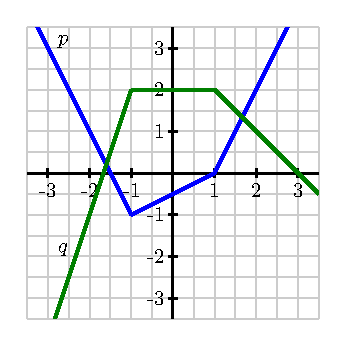
\includegraphics[scale=.75]{figures/2_1_Ez3.eps}
\end{center}
\ba
	\item Let $r(x) = p(x) \cdot q(x)$.  Determine $r'(-2)$ and $r'(0)$.
	\item Are there values of $x$ for which $r'(x)$ does not exist?  If so, which values, and why?
	\item Find an equation for the tangent line to $y = r(x)$ at the point $(2,r(2))$.
	\item Let $z(x) = \frac{q(x)}{p(x)}$.  Determine $z'(0)$ and $z'(2)$.
	\item Are there values of $x$ for which $z'(x)$ does not exist?  If so, which values, and why?	
\ea

\item A farmer with large land holdings has historically grown a wide variety of crops.  With the price of ethanol fuel rising, he decides that it would be prudent to devote more and more of his acreage to producing corn.  As he grows more and more corn, he learns efficiencies that increase his yield per acre.  In the present year, he used 7000 acres of his land to grow corn, and that land had an average yield of 170 bushels per acre.  At the current time, he plans to increase his number of acres devoted to growing corn at a rate of 600 acres/year, and he expects that right now his average yield is increasing at a rate of 8 bushels per acre per year.  Use this information to answer the following questions.
\ba
	\item Say that the present year is $t = 0$, that $A(t)$ denotes the number of acres the farmer devotes to growing corn in year $t$, $Y(t)$ represents the average yield in year $t$ (measured in bushels per acre), and $C(t)$ is the total number of bushels of corn the farmer produces.  What is the formula for $C(t)$ in terms of $A(t)$ and $Y(t)$?  Why?
	\item What is the value of $C(0)$?  What does it measure?
	\item Write an expression for $C'(t)$ in terms of $A(t)$, $A'(t)$, $Y(t)$, and $Y'(t)$.  Explain your thinking.
	\item What is the value of $C'(0)$?  What does it measure?
	\item Based on the given information and your work above, estimate the value of $C(1)$.	
\ea

\item Let $f(v)$ be the gas consumption (in liters/km) of a car going at velocity $v$ (in km/hour). In other words, $f(v)$ tells you how many liters of gas the car uses to go one  kilometer if it is traveling at $v$ kilometers per hour. In addition, suppose that $f(80)=0.05$ and $f'(80) = 0.0004$.
\ba
	\item Let $g(v)$ be the distance the same car goes on one liter of gas at velocity $v$.  What is the relationship between $f(v)$ and $g(v)$? Hence find $g(80)$ and $g'(80)$.
      	\item Let $h(v)$ be the gas consumption in liters per hour of a car going at velocity $v$. In other words, $h(v)$ tells you how many liters of gas the car uses in one hour if it is going at velocity $v$.   What is the algebraic relationship between $h(v)$ and $f(v)$?  Hence find $h(80)$ and $h'(80)$.     
	\item How would you explain the practical meaning of these function and derivative values to a driver who knows no calculus?  Include units on each of the function and derivative values you discuss in your response.  
\ea

\item An object moving vertically has its height at time $t$ (measured in feet, with time in seconds) given by the function $h(t) = 3 + \frac{2\cos(t)}{1.2^t}$.
\ba
	\item What is the object's instantaneous velocity when $t =2$?
	\item What is the object's acceleration at the instant $t = 2$?
	\item Describe in everyday language the behavior of the object at the instant $t = 2$.
\ea

\item Let $f(x) = \sin(x) \cot(x)$.
\ba
	\item Use the product rule to find $f'(x)$.
	\item True or false: for all real numbers $x$, $f(x) = \cos(x)$.
	\item Explain why the function that you found in (a) is almost the opposite of the sine function, but not quite.  (Hint: convert all of the trigonometric functions in (a) to sines and cosines, and work to simplify.  Think carefully about the domain of $f$ and the domain of $f'$.)
\ea
\end{enumerate}

%---------------------------------------------
% END OF EXERCISES ON SECOND PAGE
%---------------------------------------------
\end{multicols*}
\end{adjustwidth*}

\afterexercises 

\cleardoublepage